% \smalltitle{سوال 1.1}
% \begin{enumerate}
%     \item \phantom{text}
%     \\
%     \begin{latin}
%         \noindent
%         $S \rightarrow aSd|X|Y|Z$\\
%         $X \rightarrow aXc|Y$\\
%         $Y \rightarrow bYc|\epsilon$\\
%         $Z \rightarrow bZd|Y$
%     \end{latin}
%     \item \phantom{text}
%     \\
%     \begin{latin}
%         $S \rightarrow ab | Xb$\\
%         $X \rightarrow a|Y$\\
%         $Y \rightarrow aXb | bXa | aXa | bXb$
%     \end{latin}
% \end{enumerate}
شکل زیر را برای حل این سوال در نظر بگیرید که در هر قسمت مشخص شده که کدامیک از وظایف، 
شاخه‌های پایینی درخت را 
prune 
کرده است.
همانطور که از شکل پیداست، هیچ‌گاه نمی‌توانیم وظایف، گفته‌شده را زمانبندی کنیم.

  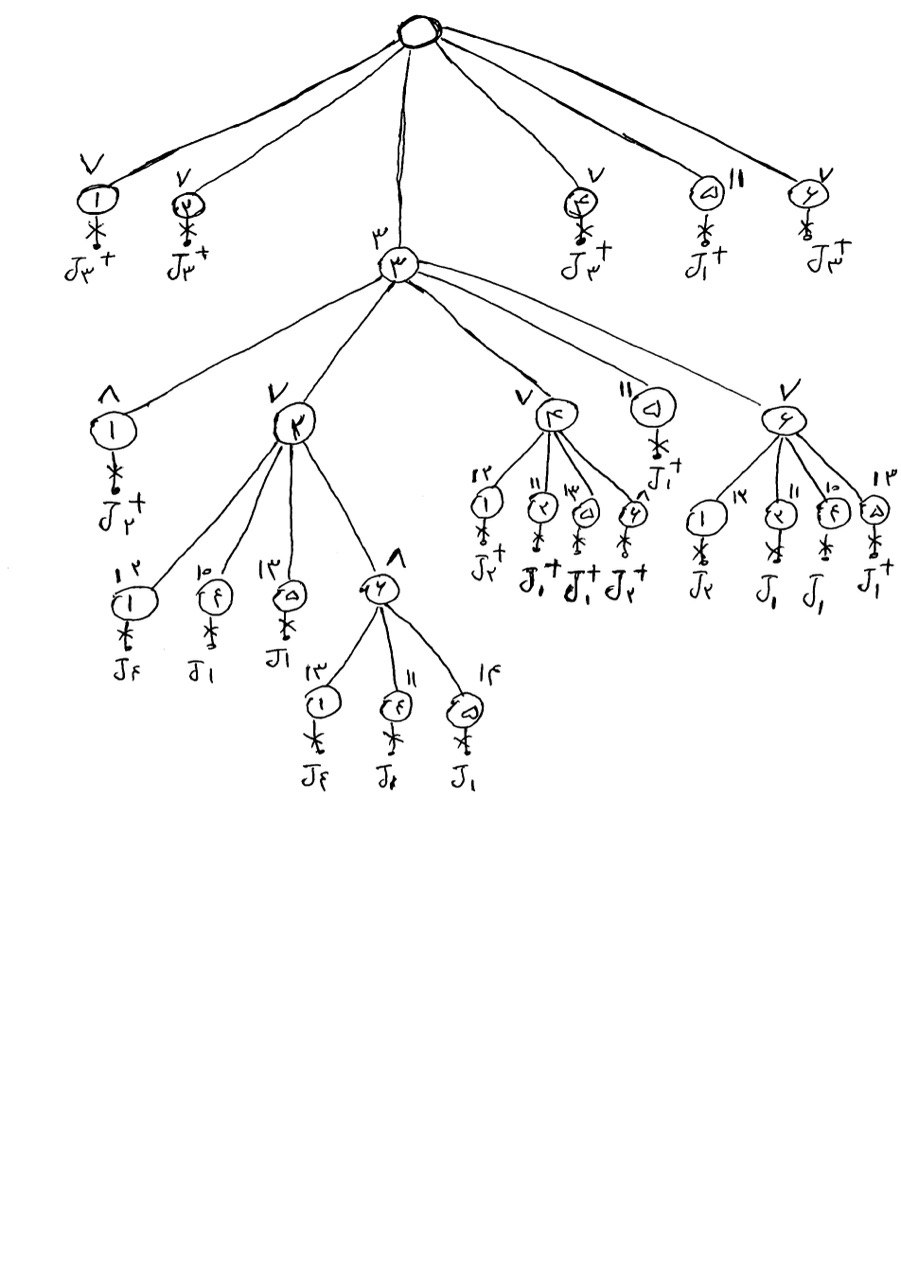
\includegraphics[scale=0.4]{pics/bratley.jpg}



% با معادلات بالا نیز می‌توان اثبات کرد 